%
\hsection{Keys}%
%
In \cref{def:entity}, we stated that an entity can be distinguished from all other entities in the world.
This means that it must be unique.
The only way it can be unique is because of its attributes.

These unique identifiers are called \emph{keys}~\cite{S2024D:CDMERDE}.%
%
\begin{definition}[Super Key]%
A \emph{super key} is an attribute or set of attributes of an entity type that unique identifies an entity in an entity set~\cite{S2024D:CDMERDE,G2011EW2ITDS:CMUTERM}.%
\end{definition}%
%
A student entity, for example, can uniquely be identified by the student ID.
It can also be uniquely identified by the combination of the address and mobile phone number.
Or just by the mobile phone number.
Or the email address.
Or by the government-issued ID.
Or we could try using the name, address, and \pgls{dateOfBirth}.%
%
\begin{definition}[Candidate Key]%
A \emph{candidate key} of an entity type is a minimal super key, i.e., a super key consisting of the smallest number of attributes~\cite{S2024D:CDMERDE,G2011EW2ITDS:CMUTERM}.%
\end{definition}%
%
We have at least three different candidate keys for students:
the student ID, the government-issued ID, and the mobile phone number.%
%
\begin{definition}[Primary Key]%
\label{sec:primaryKey}%
The \emph{primary key} of an entity type is a \emph{candidate key} that is used when modeling relationships between different entity types.%
\end{definition}%
%
Later in our \db\ design, we will also model how students enroll into modules.
Then we will have another entity type for modules.
It will be necessary to establish relationships between student and module entities.
We will need one primary key that is used to uniquely identify students.
Which of the candidate keys makes the most sense?

Phone numbers may change.
Primary keys should never change.
Also, a student may have multiple phone numbers.
This would feel awkward to use a primary key.
Actually, some students might not have a mobile phone number.
This may be rare, but it could happen, as we already discussed before.
Primary keys should never be \sqlilIdx{NULL}.
So we rule out phone numbers as primary keys.
This leaves us the government-issued ID and the student~ID that the university itself issues.

We would naturally prefer the student ID.
The reason is as follows:
A student joins a curriculum, maybe studies in the Bachelor Program \inQuotes{Computer Science and Technology} at our university.
For this process, they receive a student~ID.
This student~ID does not just represent them as a person, but it represents them \inQuotes{as a person in the function \inQuotes{BSc student of Computer Science and Technology.}}
Later, after graduation, they may join a Master's program and get a new, different student~ID.
This realization makes us feel a bit anxious about or concept of modeling students\dots

But there is another compelling and potentially more alarming reason to \emph{not} use the ID number as primary key:
Foreign exchange students, so-called 留学生, do not have IDs issued by the Chinese government.
As said, primary keys should never be \sqlilIdx{NULL}, so we rule out government-issued IDs as well.

Another criterion for primary keys is that they should be reasonably small.
For example, composite attributes or attributes that consist of longer texts are not very suitable.
The reason is that much later, in our logical \db\ design step, we will often create tables to represent the relationships between entity types.
Recall, for example, our \sqlil{demand} table from back in \cref{sec:factory:demand}.
This means that primary keys are not just stored as part of their original entities, but also as part of all of the relations they are involved in.
While this is a technological aspect that does not really belong into the conceptual schema design stage, it is something that we should keep in mind:
Huge keys are bad.
In summary:%
%
\bestPractice{primaryKeys}{%
Primary keys should:%
\begin{enumerate}%
\item be unique for each entity~(obviously),%
\item be immutable over the lifetime of an entity,%
\item not be optional, i.e., they should never be allowed to be \sqlilIdx{NULL},%
\item not be derived attributes,%
\item always be single-valued attributes, i.e., not be multi-valued attributes,%
\item consist of single attributes, i.e., not be based on candidate keys consisting of multiple attributes,%
\item be simple attributes, i.e., not composed attributes,%
\item be small in terms of the expected required storage size~(see also \cref{bp:surrogatePrimaryKey}).%
\end{enumerate}%
}%
%
Sometimes, it can happen that we end up with entity types where \emph{no} suitable primary key exists.
Maybe all the attributes that form candidate keys are just too long.
In such a case, we can use a technique we already learned in back in \cref{sec:factory:table:product}:%
%
\begin{definition}[Surrogate Key]%
\label{def:surrogateKey}%
When no suitable candidate key for an entity exists, an artificial key, such as an auto-incremented integer value, can be used as \emph{surrogate key}.%
\end{definition}%
\begin{figure}%
%
\centering%
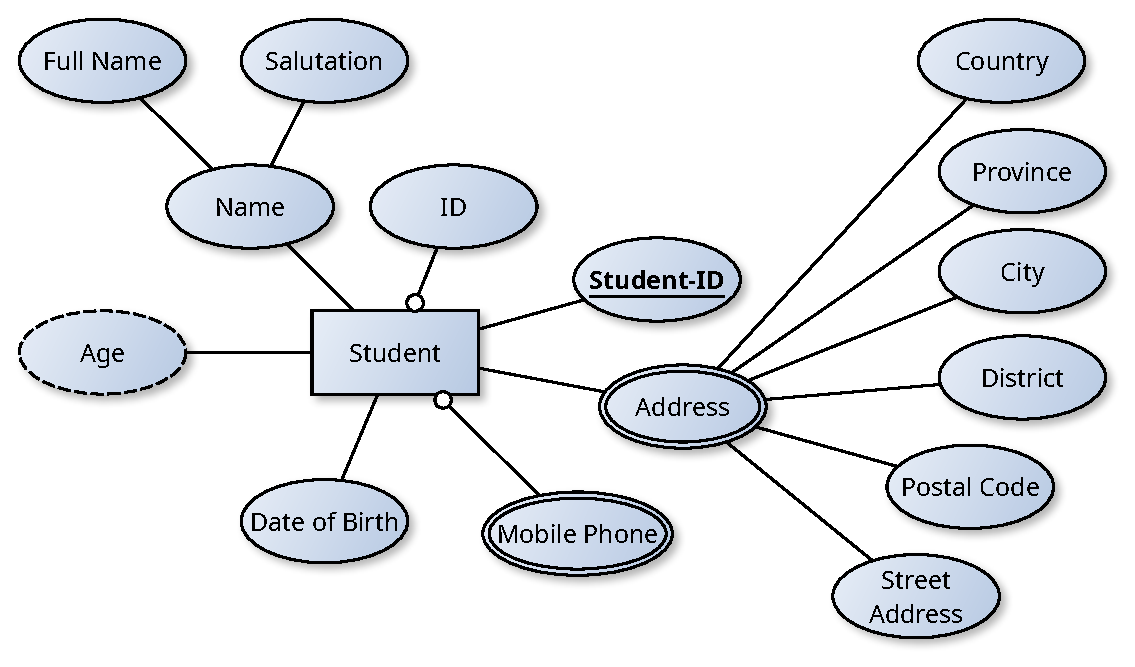
\includegraphics[scale=0.6]{\currentDir/erdStudent5}%
\caption{A new version of the \emph{Student} \pgls{ERD} from \cref{fig:erdStudent4}, this time with \emph{Student-ID} marked as primary key.}%
\label{fig:erdStudent5}%
\end{figure}%
%
While we feel very pessimistic about our idea about the concept of students, for now, we bravely march on and update our \pgls{ERD} from \cref{fig:erdStudent4}.
In the new \cref{fig:erdStudent5}, the attribute \emph{Student-ID} is marked as primary key.
This is done by underlining the attribute name~\cite{G2011EW2ITDS:CMUTERM}.%
%
\FloatBarrier%
\endhsection%
%
